\documentclass[usenames,dvipsnames]{beamer}

\usepackage{graphicx,url}
\usepackage[utf8]{inputenc}
%\batchmode
% \usepackage{pgfpages}
% \pgfpagesuselayout{4 on 1}[letterpaper,landscape,border shrink=5mm]
\usepackage{amsmath,amssymb,enumerate,epsfig,calc,xcolor,ifthen}
\usetheme{CambridgeUS}
\usecolortheme{crane}

\usepackage{empheq}


\usepackage{xcolor}
\definecolor{applegreen}{rgb}{0.55, 0.71, 0.0}
\definecolor{awesome}{rgb}{1.0, 0.13, 0.32}
\colorlet{enum1}{green}
\colorlet{enum2}{applegreen}
\colorlet{enum3}{orange}
\usepackage[most]{tcolorbox}

\tcbset{
    frame code={}
    center title,
    left=0pt,
    right=0pt,
    top=0pt,
    bottom=0pt,
    colback=blue!70,
    colframe=white,
    width=\dimexpr\textwidth\relax,
    enlarge left by=0mm,
    boxsep=5pt,
    arc=15pt,outer arc=15pt,
    }
    
\usepackage{tikz,etoolbox}
\newcommand*\mylogo{%
  \renewcommand*\do[1]{\includegraphics[height=8mm]{##1}}
  \dolistloop\mylogolist}
\newcommand*\setmylogo[1]{%
  \renewcommand*\mylogolist{}%
  \forcsvlist{\listadd\mylogolist}{#1}}
\newcommand*\addlogoleft[1]{%
  \global\let\oldmylogolist\mylogolist
  \renewcommand*\mylogolist{}%
  \forcsvlist{\listadd\mylogolist}{#1}%
  \forcsvlist{\listeadd\mylogolist}{\oldmylogolist}}
\newcommand*\addlogoright[1]{%
  \forcsvlist{\listadd\mylogolist}{#1}}
\newcommand*\mylogolist{}


\usetikzlibrary{shapes.arrows}

\def\deltaD{{D_1}}
\def\comment#1{\par\noindent\llap{$\Rightarrow$\enskip}{\bf #1}\par}
\newcommand{\bfv}{\mbox{\boldmath$v$}}
\newcommand{\bfx}{\mbox{\boldmath$x$}}
\newcommand{\bfk}{\mbox{\boldmath$k$}}
\newcommand{\bfp}{\mbox{\boldmath$p$}}
\newcommand{\bfq}{\mbox{\boldmath$q$}}
\newcommand{\bfr}{\mbox{\boldmath$r$}}
\newcommand{\bfu}{\mbox{\boldmath$u$}}
\newcommand{\bfPhi}{\mbox{\boldmath$\Phi$}}
\newcommand{\bfM}{\mbox{\boldmath$M$}}
\newcommand{\fnl}{f_{\rm NL}}
\newcommand{\gnl}{g_{\rm NL}}
\newcommand{\tdu}{\widetilde{u}}
\newcommand{\tdPhi}{\widetilde{\Phi}}
\newcommand{\tdG}{\widetilde{G}}
\newcommand{\tdP}{\widetilde{P}}
\newcommand{\tdR}{\widetilde{R}}




\definecolor{gold}{rgb}{0.95, 0.85, 0.12}

\newcommand\widecolourbox[1]{{\setlength\fboxrule{1pt}\setlength\fboxsep{8pt}\fcolorbox{red}{applegreen}{\enspace#1\enspace }}}

\newcommand\widecolourboxx[1]{{\setlength\fboxrule{1pt}\setlength\fboxsep{8pt}\fcolorbox{applegreen}{awesome}{\enspace#1\enspace }}}


\newcommand\widecolourboxxx[1]{{\setlength\fboxrule{1pt}\setlength\fboxsep{8pt}\fcolorbox{black}{orange}{\enspace#1\enspace }}}


\makeatletter
\newcommand*{\IfColorUndefined}[1]{%
  \begingroup
    \escapechar=`\\ %
    \expandafter\expandafter\expandafter
  \endgroup
  \expandafter\ifx\csname\string\color @#1\endcsname\relax
    \expandafter\@firstoftwo
  \else
    \expandafter\@secondoftwo
  \fi
}
\makeatother


\tikzset{
    myarrow/.style={
        draw,
        fill=orange,
        single arrow,
        minimum height=3.5ex,
        single arrow head extend=1ex
    }
}
\newcommand{\arrowleft}{%
\tikz [baseline=-0.5ex]{\node [myarrow,rotate=-110] {};}
}
\newcommand{\arrowright}{%
\tikz [baseline=-0.5ex]{\node [myarrow,rotate=-70] {};}
}

\newcommand{\arrowdown}{%
\tikz [baseline=-0.5ex]{\node [myarrow,rotate=-90] {};}
}
\usepackage{tikzsymbols}



\title{ {\color{awesome} Machine Learning}}
\author{\color{awesome} \bf Ben Bose}
%\institute{}
%\date{ \color{awesome} \bf  \today} 
\begin{document}


 \addtobeamertemplate{frametitle}{}{%
    \begin{tikzpicture}[remember picture,overlay]
      \node[anchor=north east,yshift=2pt] at (current page.north east) {\mylogo};
    \end{tikzpicture}}
    

\begin{frame}
 \begin{tcolorbox}
 \centering
 {\bf \Huge \color{orange} {\bf \color{awesome}  Machine Learning 2:} Optimisation and good practices \\ }  
 \end{tcolorbox}
 \centering
    \includegraphics[width=8cm,height=5cm]{figs/gp.png}
\end{frame}

\begin{frame}
\centering
{\bf How do we improve a ML algorithm?} 
\begin{itemize}
\item 
More training examples.\pause
\item 
Less features that fits training set equally well. \pause
\item 
More features to fit the training set better. \pause
\item 
Choose features more carefully. \pause 
\item 
Regularisation 
\end{itemize}
\end{frame}

\begin{frame}
 \centering
 {\bf Regularisation } \\ \pause
    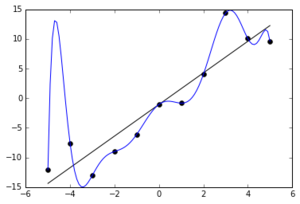
\includegraphics[width=5cm,height=3cm]{figs/biasvsvar.png} 
        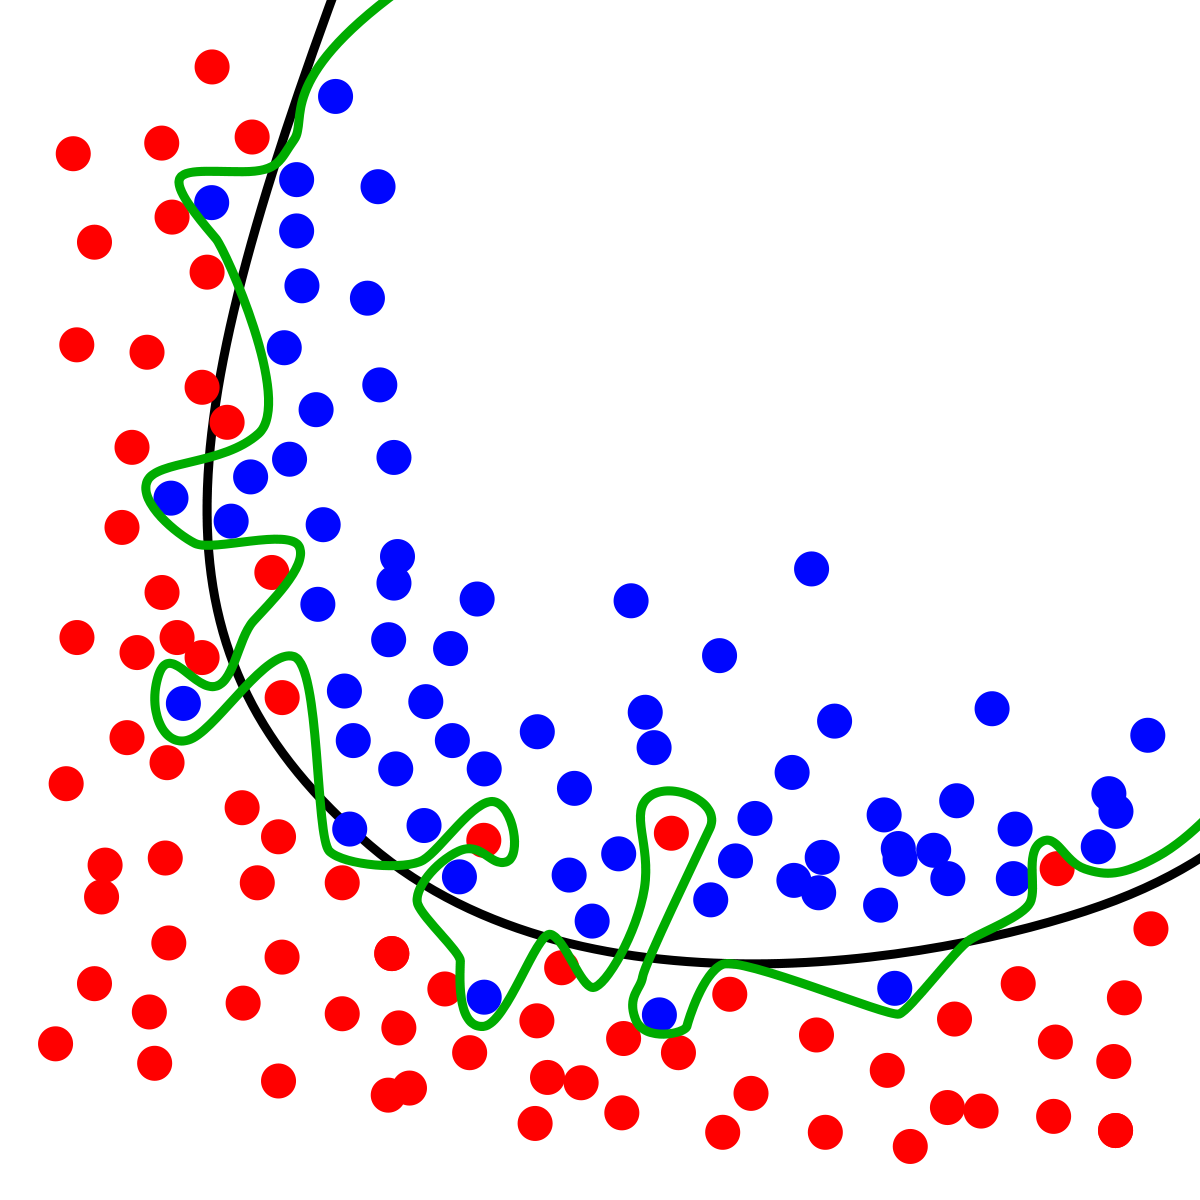
\includegraphics[width=5cm,height=3cm]{figs/overfit2.png} \\ \pause

    \begin{itemize}
    \item
   Too many features lets $h(\theta^T x)$ fit the data very well, but would fail to generalise --- {\bf \color{red} overfitting/ high variance}. \pause
   \item 
   Too few features and $h(\theta^T x)$ would fail to fit the data well and have a large error ---  {\bf \color{red} underfitting/ high bias}.\pause
 \end{itemize}
 {\bf Options to cure overfitting/ high variance: }
     \begin{enumerate}
    \item
	Reduce number of features .... manually ??, use some model selection algorithm ?? \pause
   \item 
	Incorporate a method that `weights' features in order of their importance --- {\bf \color{orange} regularisation}. 
 \end{enumerate}
\end{frame}

\begin{frame}
Regularisation can just be added as a term in the cost function .... 
\begin{equation}
J(\theta) = \frac{1}{m} \sum_{i=1}^m \left[ y^i \log[h({\bf \theta^T x^i})] + (1-y^i)\log[1-h({\bf \theta^T x^i})] \right] + \lambda \theta^T\theta . \pause
\end{equation}
{\bf Regularisation parameter } $\lambda$ needs to be chosen carefully \\ \quad \\
$\lambda$ too small and regularisation becomes useless.  \\
$\lambda$ too large and we get underfitting. \\ \quad \\ \pause
How do we choose value in practice? \\ 
\end{frame}

\begin{frame}
{\bf Cross-validation and test sets}   \pause
{\bf \large How do we test a given ML algorithm or choice of $\lambda$ ? } \pause \\ \quad \\

\begin{enumerate}
\item
Split data roughly into three sets: 
\begin{itemize}
\item 
{\color{red} Training} set $\approx  60\%$ 
\item 
{\color{red} Cross-validation} set $\approx  20\%$  
\item
{\color{red} Test} set $\approx  20\%$ 
\end{itemize}
\pause
\item 
Calculate hypothesis fits ($\theta$) using training set. \pause
\item 
Calculate error of each algorithm using the CV set. Choose best algorithm ($\lambda$ value or model).  \footnote{done w/o regularisation!}   \pause 
\item
Calculate the error on the test set to confirm choice. 
\end{enumerate}
\end{frame}

\begin{frame}{Diagnosing bias and variance - dimension}
\centering
    \includegraphics[width=12cm,height=7cm]{figs/curves_dim1.pdf} 
\end{frame}

\begin{frame}{Diagnosing bias and variance - dimension}
\centering
    \includegraphics[width=12cm,height=7cm]{figs/curves_dim2.pdf} 
\end{frame}

\begin{frame}{Diagnosing bias and variance - $\lambda$}
\centering
    \includegraphics[width=12cm,height=7cm]{figs/curves_l1.pdf} 
\end{frame}

\begin{frame}{Diagnosing bias and variance - $\lambda$}
\centering
    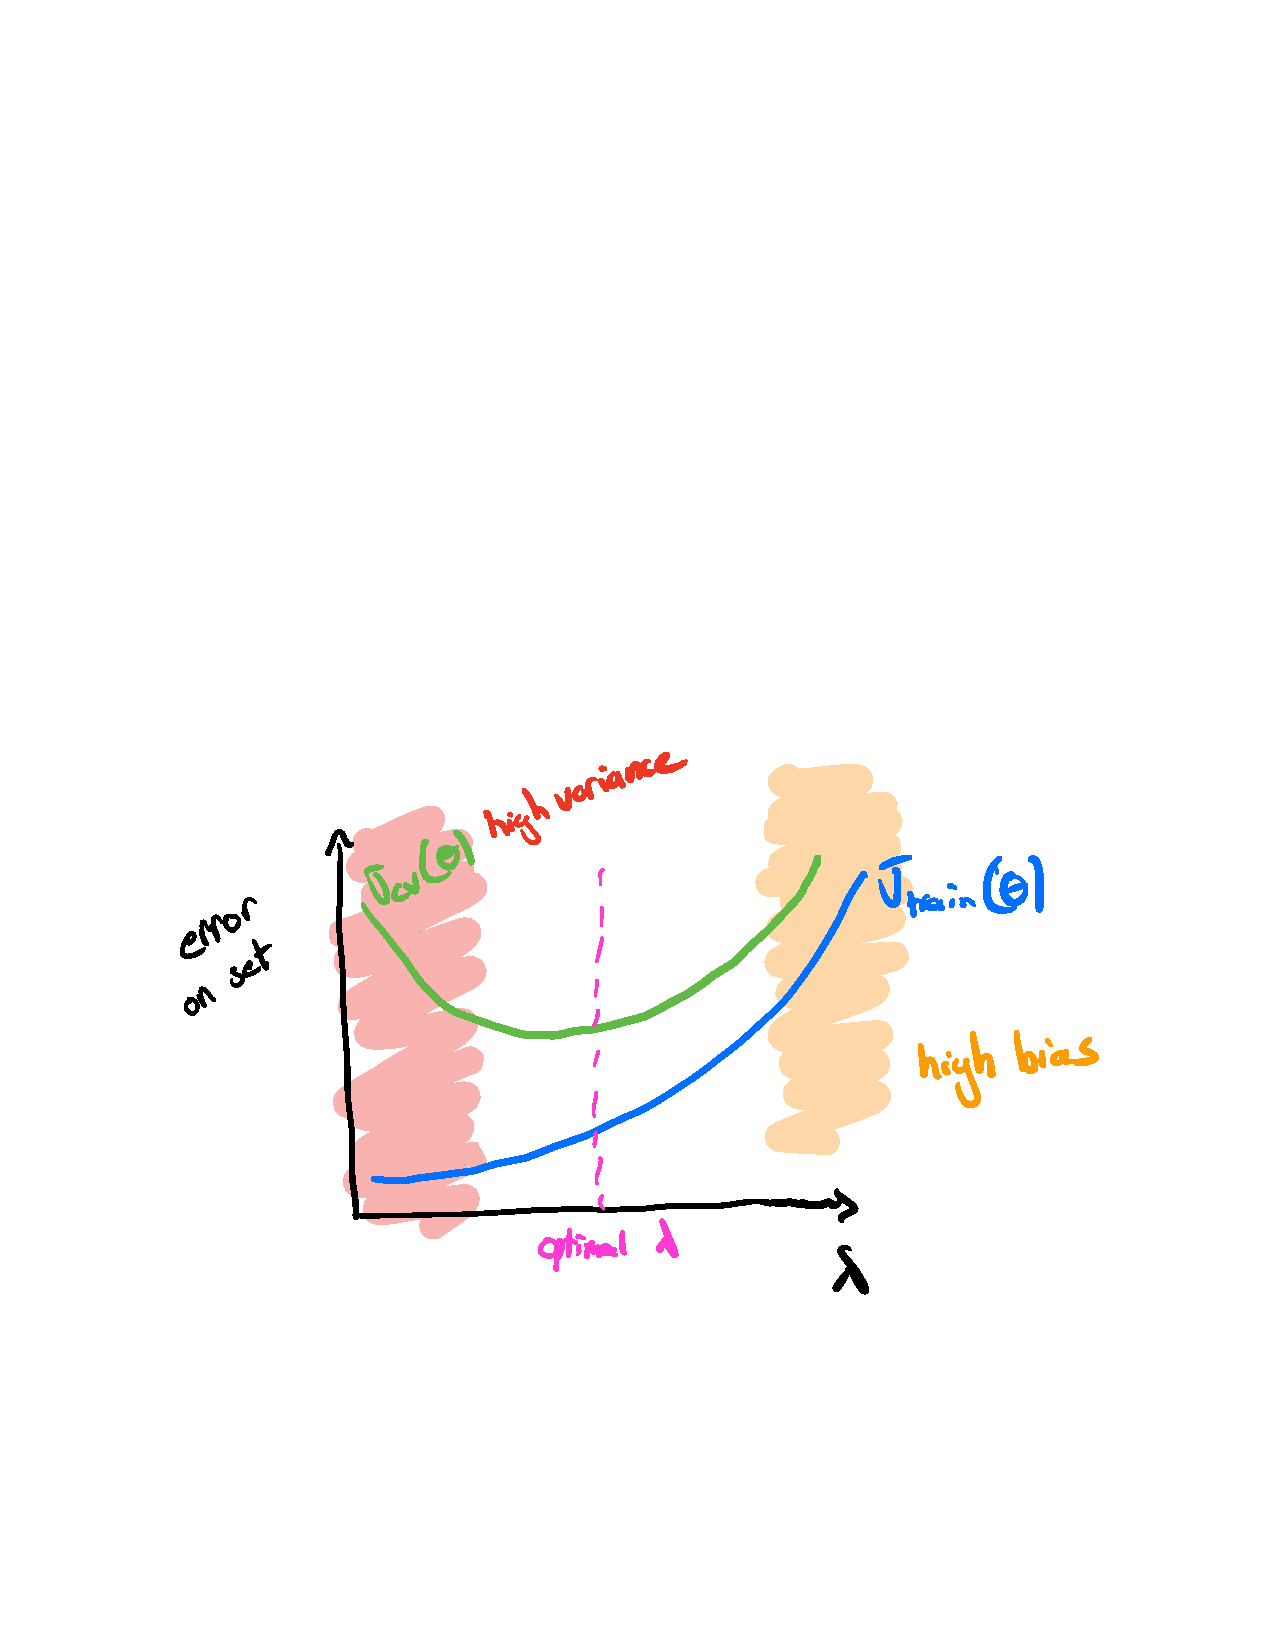
\includegraphics[width=12cm,height=7cm]{figs/curves_l2.pdf} 
\end{frame}

\begin{frame}{Diagnosing bias and variance - $\lambda$}
\centering
    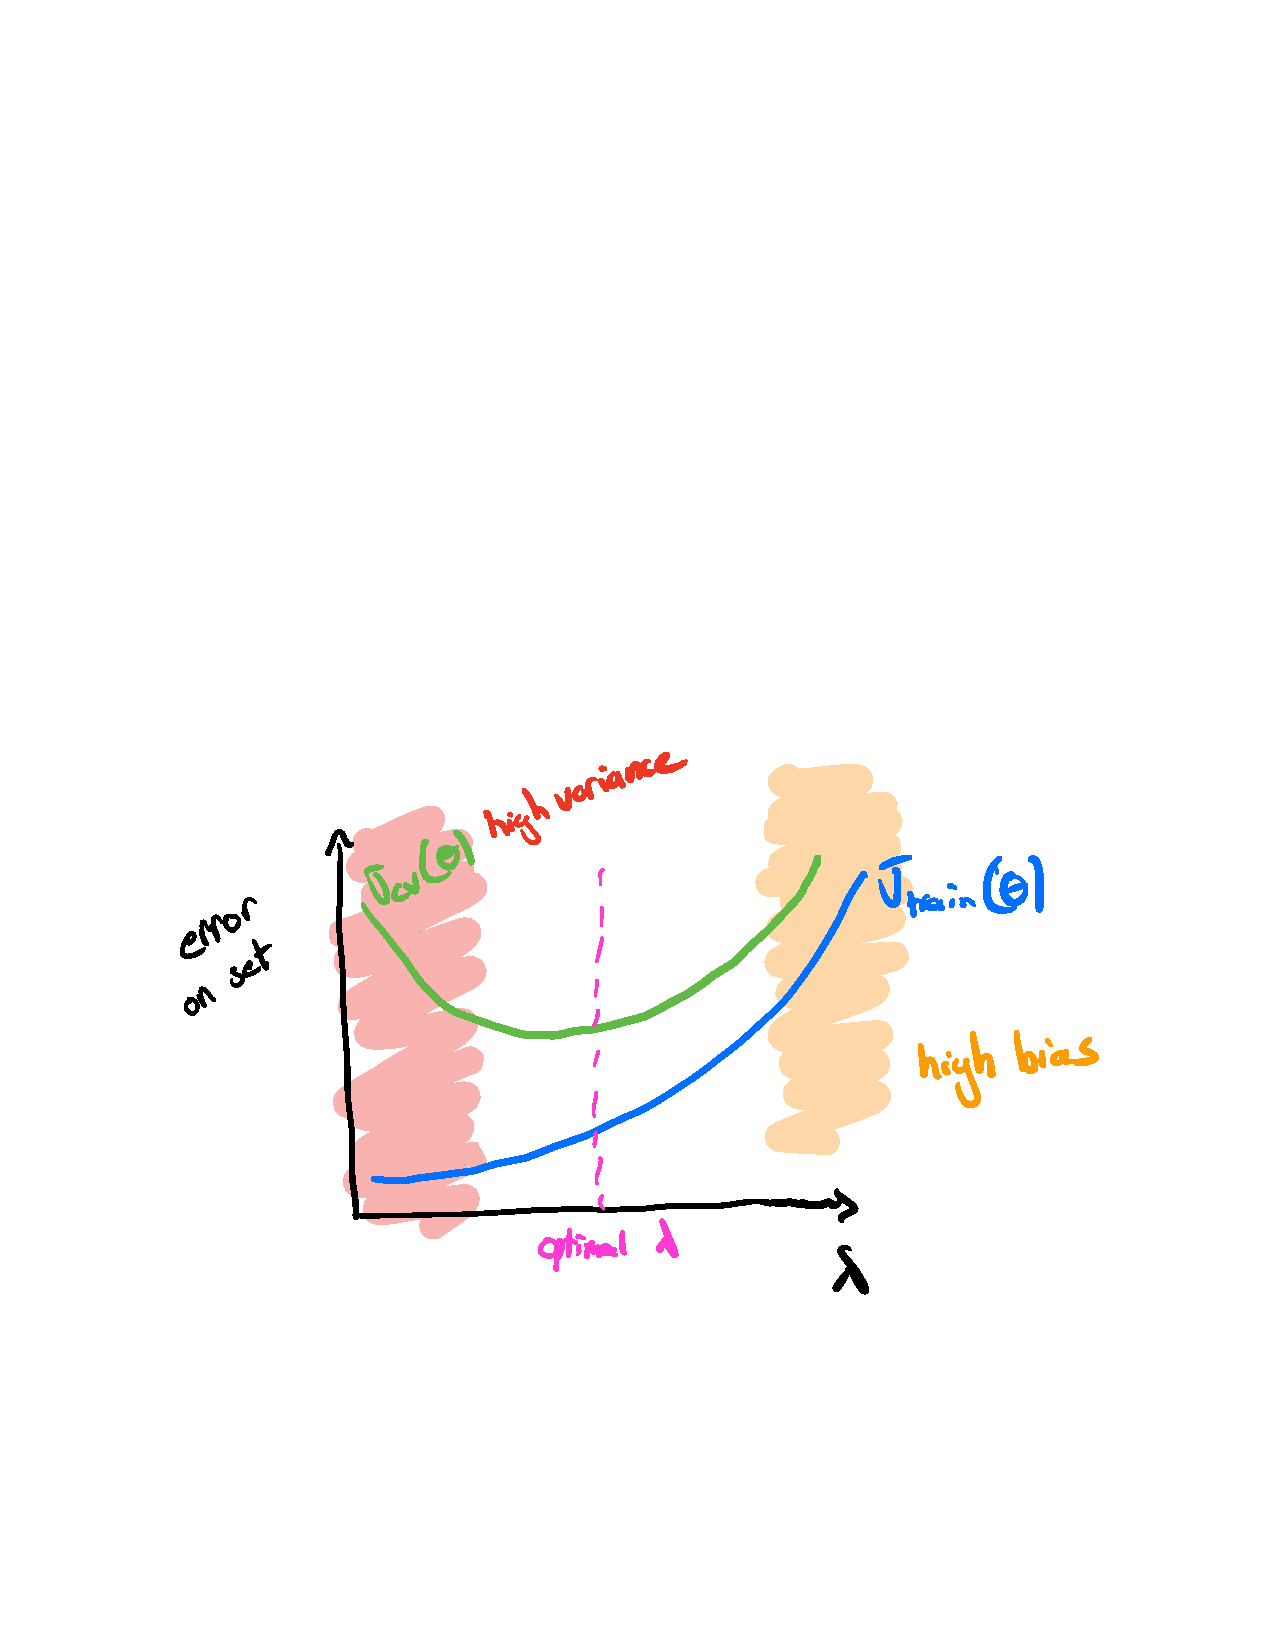
\includegraphics[width=12cm,height=7cm]{figs/curves_l2.pdf} 
\end{frame}


\begin{frame}{Diagnosing bias and variance - $\lambda$}
\centering
    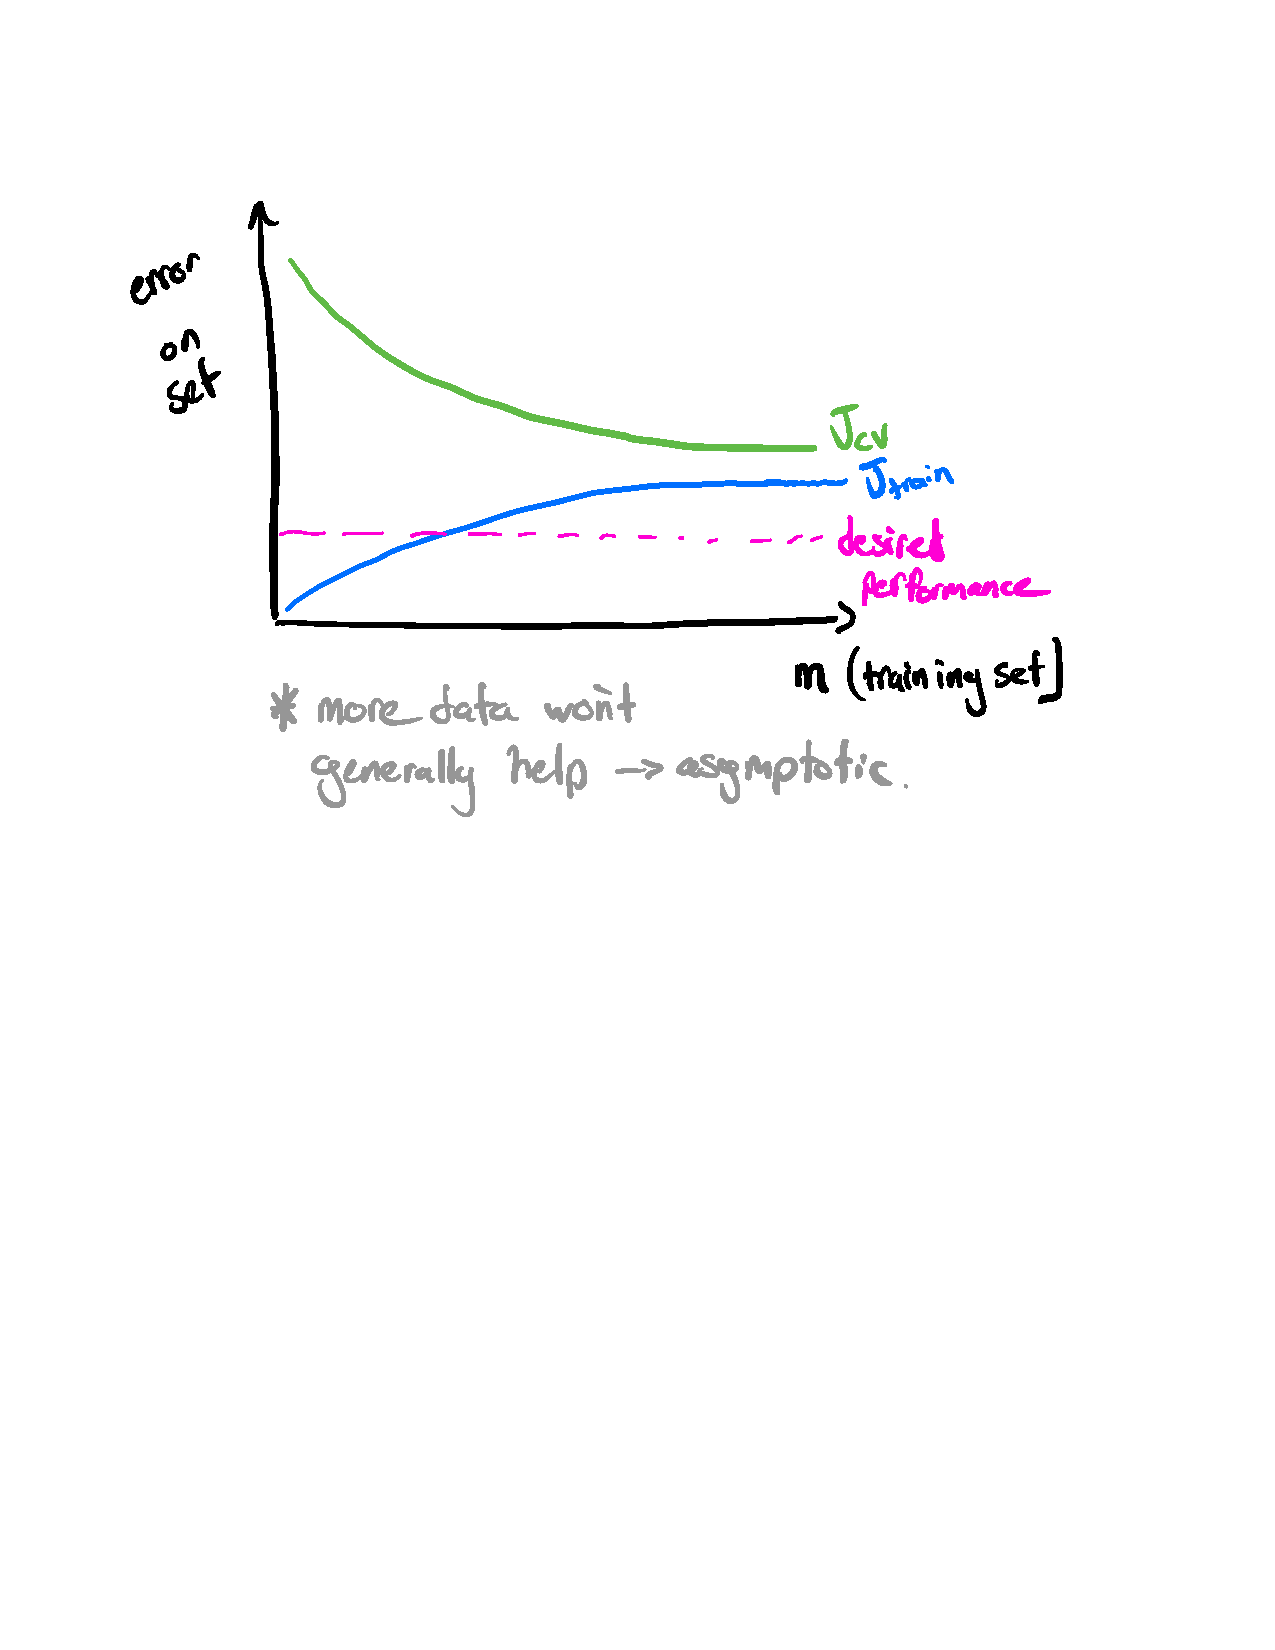
\includegraphics[width=12cm,height=7cm]{figs/curves_lc1.pdf} 
\end{frame}

\begin{frame}{Diagnosing bias and variance - $\lambda$}
\centering
    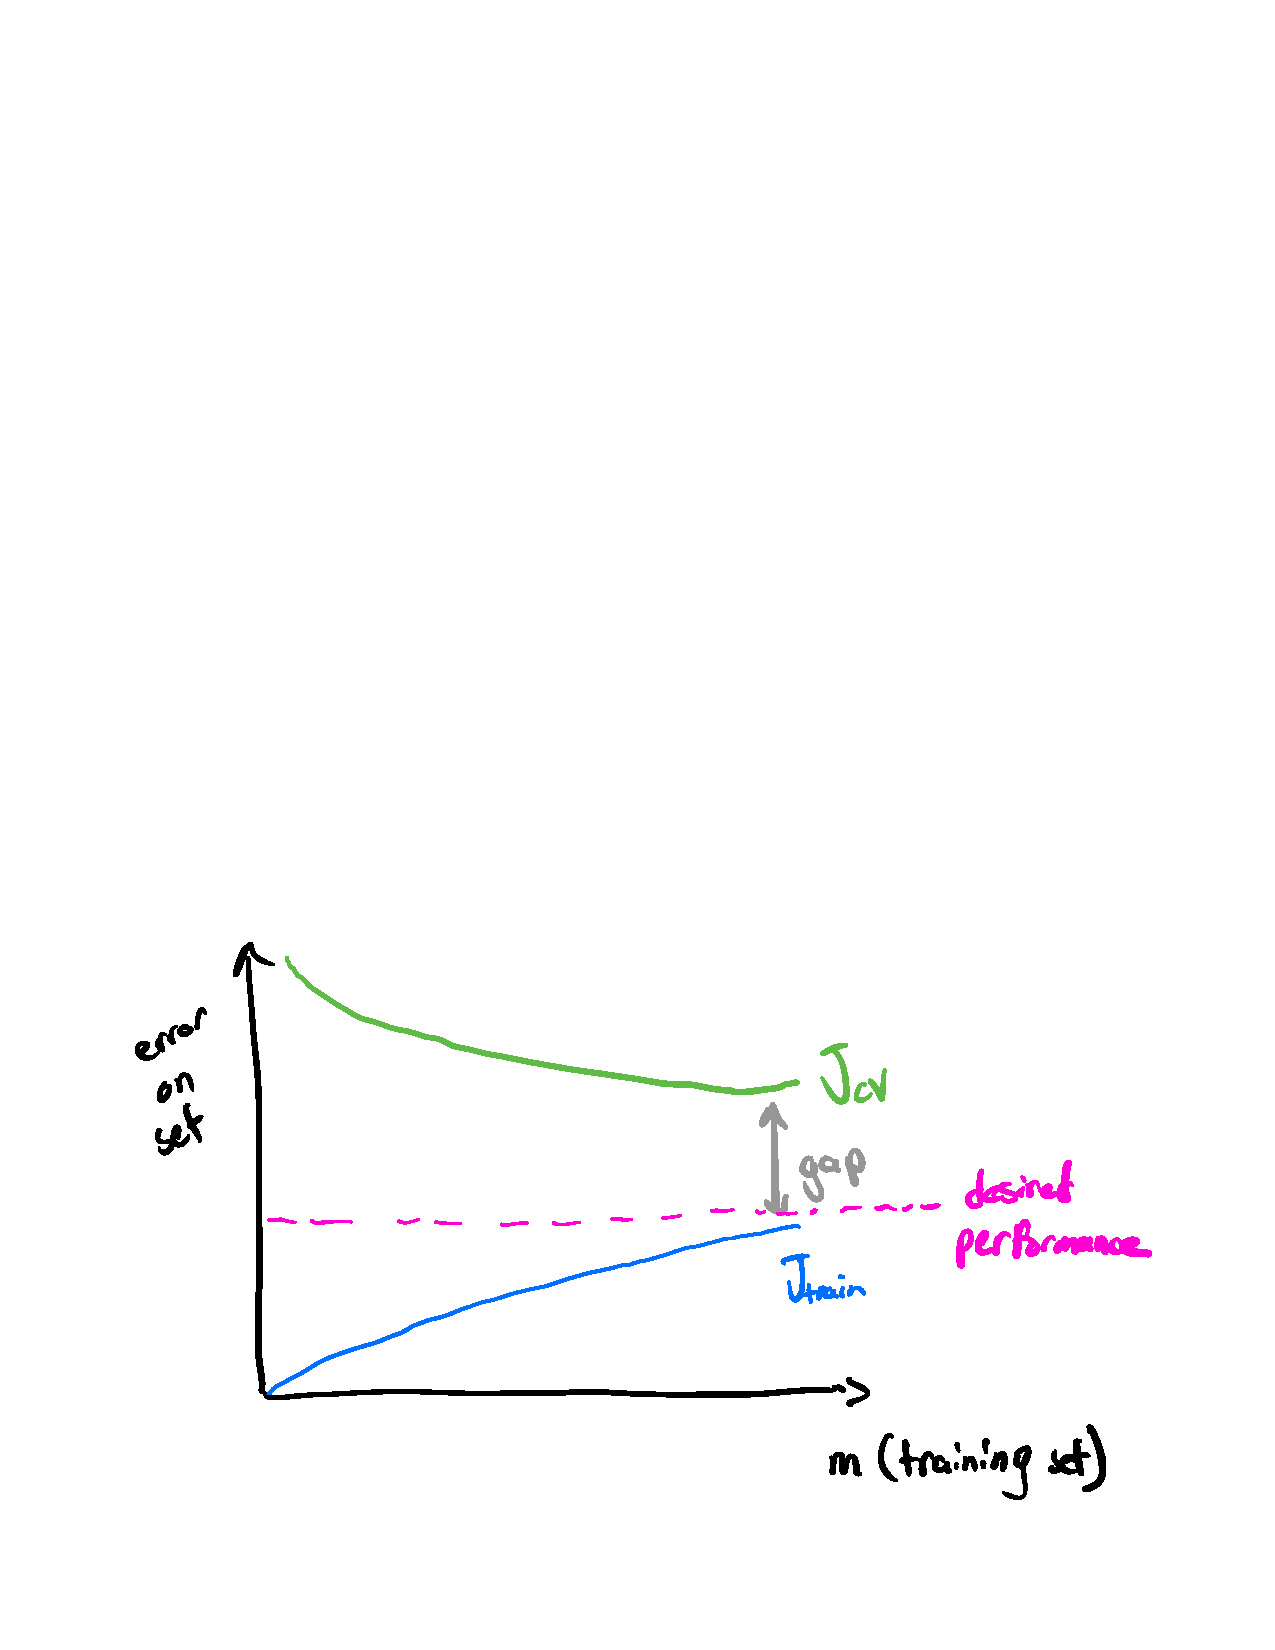
\includegraphics[width=12cm,height=7cm]{figs/curves_lc2.pdf} 
\end{frame}



\begin{frame}
\centering
{\bf How do we improve a ML algorithm?} 
\begin{itemize}
\item 
More training examples. -{\color{green} fixes high variance } \pause
\item 
Less features that fits training set equally well. -{\color{green} fixes high variance } \pause
\item 
More features to fit the training set better. -{\color{green} fixes high bias } \pause
\item 
Regularisation:  increase $\lambda$ -{\color{green} fixes high variance } \pause
\item
Regularisation:  decrease $\lambda$ -{\color{green} fixes high bias } \pause
\item
{\bf Choose features more carefully!   }
\end{itemize}
\end{frame}


\begin{frame}{ML-Flow and Error Analysis}
{\bf \large How to approach an ML problem?}


\begin{enumerate}
\item Take a look at your data and pre-process them
\item
Quick and dirty algorithm to get some predictions. 
\item 
Plot learning curves to inspire  accuracy improvement.
\item
Error analysis --- {\bf requires a well defined error-metric! }
\end{enumerate}
 One can use the obvious metric :
 \begin{equation}
 Error = \frac{1}{m_{set}} \sum_{i=1}^{m_{set}} err(h(\theta^T x^i), y^i),
 \end{equation}
 where 
  \[   
err(h(\theta^T x^i), y^i) = 
     \begin{cases}
       1 &\quad\text{$h({ \theta^T x^i})_{y=0}$ } \ge 0.5  \quad  OR \quad   \text{$h({ \theta^T x^i})_{y=1}$ }  < 0.5  \\
       0 &\quad\text{otherwise}\\
     \end{cases} \quad ,
\]
\end{frame}

\begin{frame}{Skewed data} 
\centering
    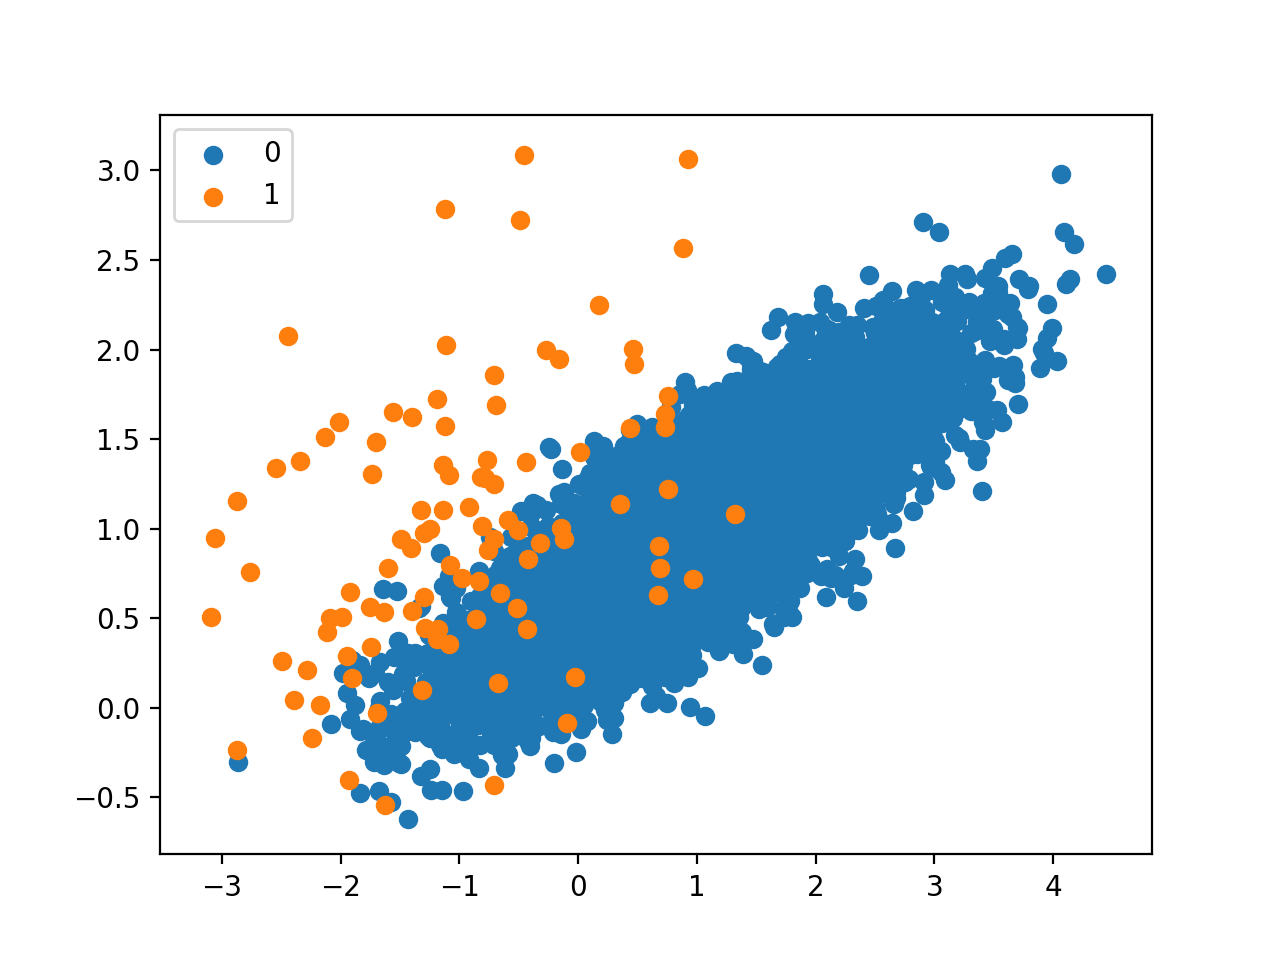
\includegraphics[width=10cm,height=6cm]{figs/skewed.png}  \\ 
    Setting $h(\theta^T x) = 0$ always will give a very low error....
\end{frame}

\begin{frame}{Precision and Recall} 
\centering
    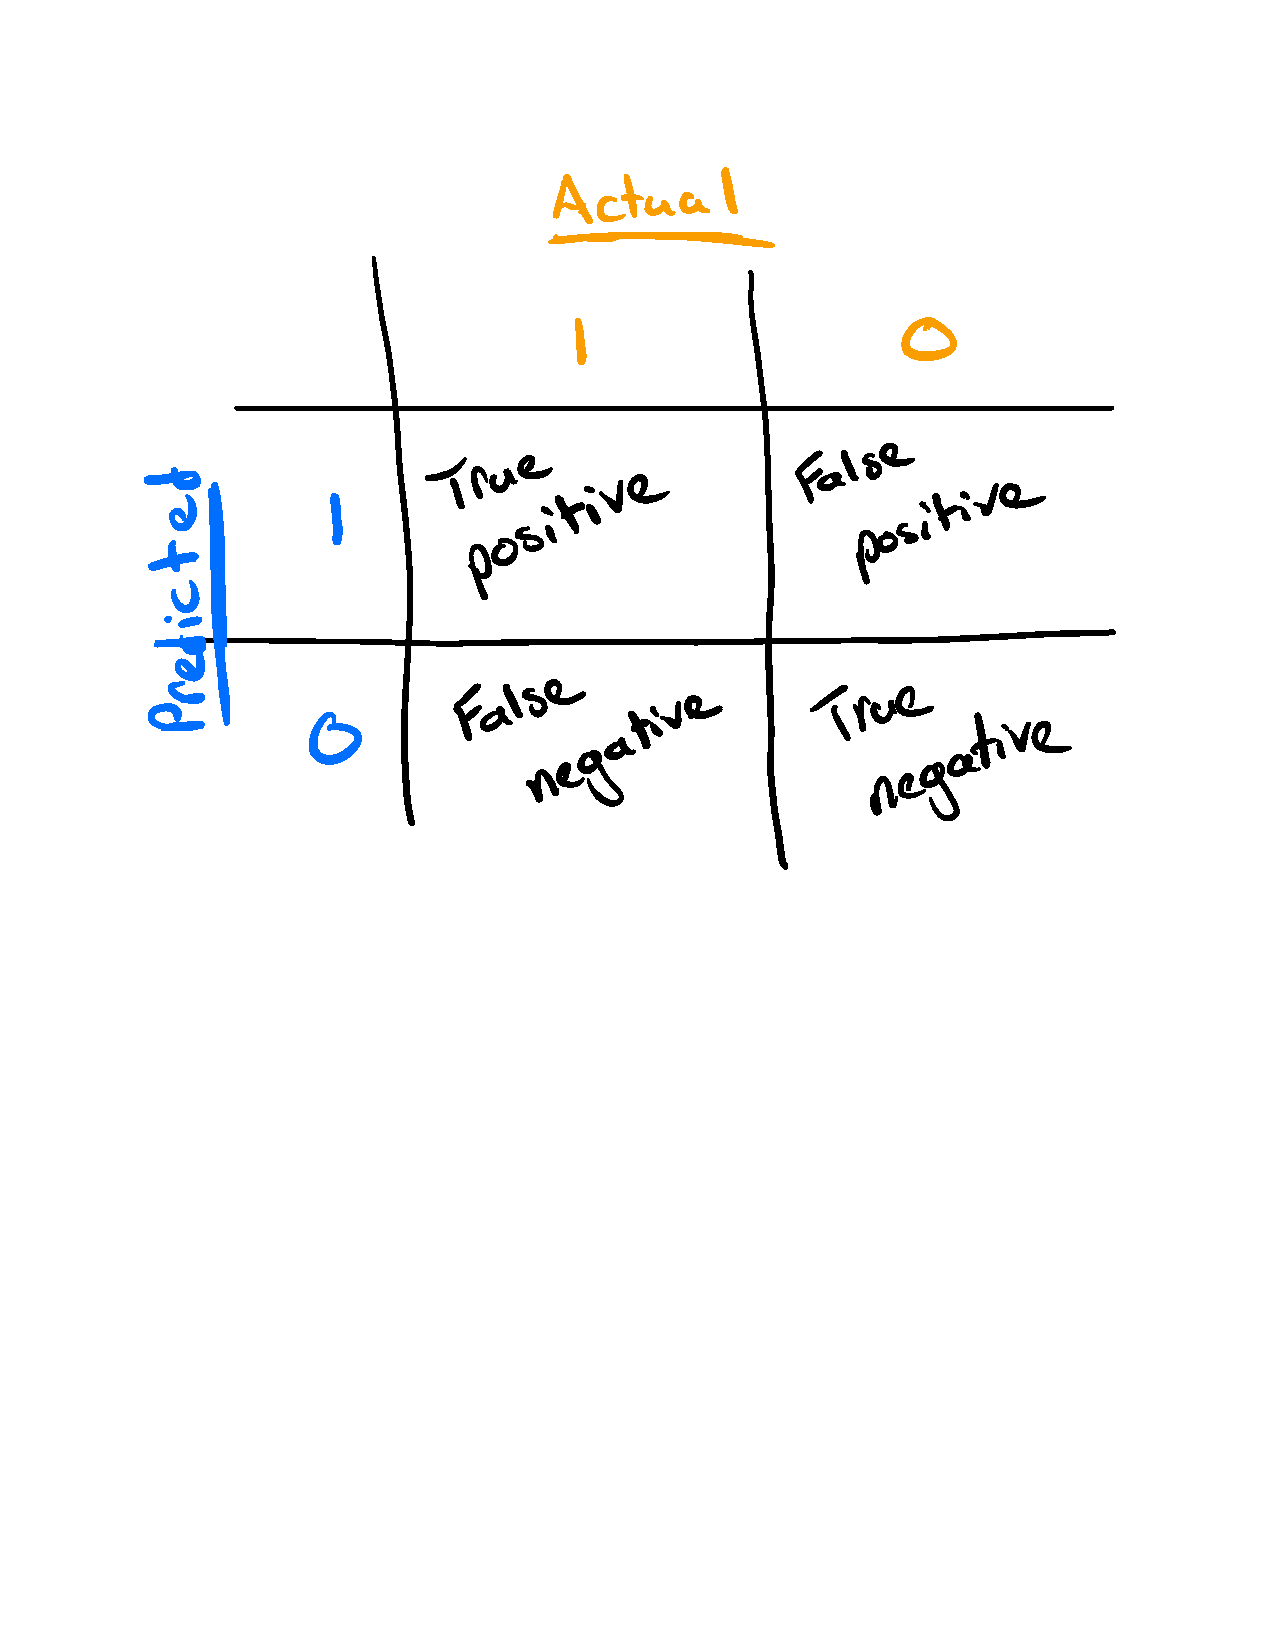
\includegraphics[width=12cm,height=4.5cm]{figs/pandr.pdf}  \\ 
    
    \begin{equation}
    Precision = \frac{\text{True Pos}}{\text{True Pos + False Pos}} , \quad \quad     Recall = \frac{\text{True Pos}}{\text{True Pos + False Neg}}
    \end{equation}
    {\bf Note:} Set rarest class to be $y=1$!
\end{frame}

\begin{frame}{Precision and Recall} 
Some notes:
\begin{itemize}
\item
We can change the threshold, $h(\theta^Tx)\geq threshold$, such that we gain or lose precision or recall.  \pause
\item 
The higher the threshold the higher the precision but the lower the recall. 
\item
One can combine the two into the {\bf \color{orange} F-score} which we try to maximise
\begin{equation}
0 \leq F_1 = \frac{ 2PR}{P+R} \leq 1
\end{equation}
\end{itemize}
\pause
{\bf Let's look at an example finally!!}

\end{frame}

\end{document}



